%-----------------------------------------------------------------------------------------------------------------
\chapter{Introdução}
\label{Ch:Introducao}
%---------------------------------------------------------------------------------------------------------------
%-----------------------------------------------------------------------------------------------------------------

\hspace{1cm}A indústria está constantemente à procura de novas soluções para melhorar os seus processos produtivos com o objetivo de se colocar à frente dos seus competidores. Se os níveis de competitividade na indústria são elevados, fruto do desenvolvimento tecnológico e da melhoria constante dos processos produtivos, é natural que surja a necessidade de desenvolvimento e melhoria constante nas organizações do setor das tecnologias da informação. A comunicação da informação em tempo útil é fundamental para que qualquer organização tenha sucesso.

\hspace{1cm}Existe a necessidade de melhorar constantemente a qualidade, a fluidez e a assertividade da comunicação. Da mesma forma exige-se melhor desempenho global das metodologias de desenvolvimento de novos processos, novos produtos e novas tecnologias.

\section{Contexto e Enquadramento}
%-----------------------------------------------------------------------------------------------------------------

\hspace{1cm}Os enormes volumes de capital monetário, humano e  de tempo investidos pelas grandes empresas tecnológicas em satisfação do consumidor, \textit{quality assurance} e redução do tempo de entrega são, provavelmente, os fatores com mais peso nas decisões tomadas pelos quadros executivos quando se trata de melhoria contínua dos processos produtivos \cite{goldratt2016goal}. Esta é uma premissa que se verifica em qualquer setor dada a transversalidade e a presença crescente da tecnologia quer em processos industriais produtivos, quer na prestação de serviços de consultoria IT, como é o caso do desenvolvimento de software. O desenvolvimento de software pode ser estruturado de várias formas e pode seguir várias metodologias. Para qualquer caso de desenvolvimento, existem as etapas de \textit{software development lifecycle} (SDLC) e de \textit{software testing lifecycle} (STLC), onde todos os eventos que consomem mais tempo do que aquele que é considerado aceitável, que sejam sistematicamente repetidos, são processos que o \textit{business} deve considerar automatizar.

\hspace{1cm}Automação de processos não é um conceito novo na indústria. O mesmo se pode aplicar ao desenvolvimento e controlo de qualidade de software. O que acontece, de um ponto de vista objetivo, é que se quer salvaguardar o negócio tomando partido de um conjunto de vantagens competitivas que permitem economizar tempo no desenvolvimento e na entrega de soluções. Tanto na fase de \textbf{SDLC} como na fase de \textbf{STLC} o ideal será a automatização de todo o processo -- excepcionando o de desenvolvimento de código -- onde os testes e a validação das fases de \textit{development}, \textit{staging} e \textit{production} é realizado de forma automática.


\hspace{1cm}Segundo o manifesto \textit{Agile} \cite{beck2001manifesto}, para o desenvolvimento de software deve ter-se em conta que podem ser considerados quaisquer tipos de mecanismos que providenciem agilidade ao sistema, em termos de flexibilidade no reajuste aos requisitos do cliente. Seguidamente, caso venham a ser aprovados, serão incluídos no projeto. Isto inclui as práticas da cultura \textit{DevOps} (ex \ref{Fig:Fig1}).

\begin{figure}[hbt!]
\centering
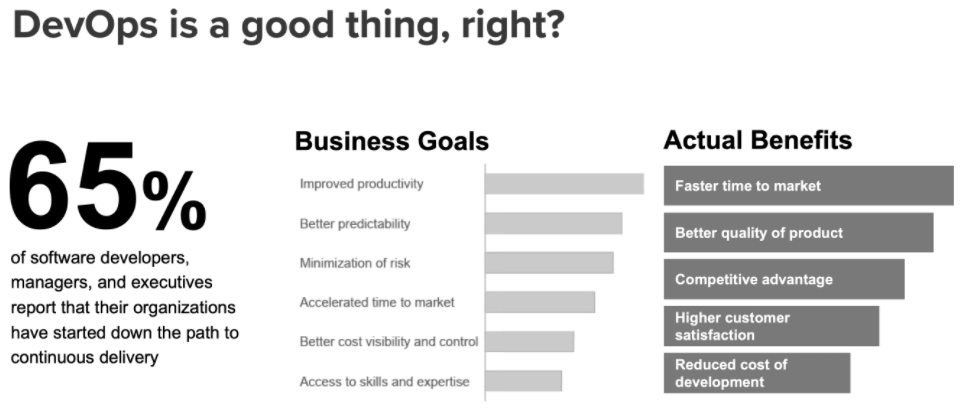
\includegraphics[width=0.9\linewidth]{Cap1/Figura1.png}
\caption{DevOps nas empresas (Fonte: Webinar -- Using VSM to Optimize DevOps Workflow)}
\label{Fig:Fig1}
\end{figure}

%-----------------------------------------------------------------------------------------------------------------
\subsection{A cultura de DevOps}

\hspace{1cm}O movimento DevOps, os seus princípios e práticas podem ser definidos de várias formas. Certos autores, como é o caso de \shortciteA{ebert2016devops}, definem este conceito através de uma visão romântica, quase utópica: \textit{``DevOps é desenvolvimento flexível e rápido, fornecendo processos de negócio. Integra eficientemente o desenvolvimento, a entrega e as operações, traduzindo-se numa ligação elegante e fluída destes três SILOS tradicionalmente separados''}. Outros autores, como \shortciteA{bass2015devops}, descrevem este conceito através de uma visão racional, focada no propósito afirmando que: \textit{``DevOps é um conjunto de práticas que têm como objetivo reduzir o tempo entre a implementação de uma mudança no sistema e a colocação dessa mesma mudança em produção normal, preservando elevada qualidade''}. Tem-se ainda, segundo o autor \shortciteA{huttermann2012devops} uma definição do conceito de DevOps mais prática e equilibrada, vejamos: \textit{``O Termo DevOps é uma mistura de desenvolvimento (representando os software developers, incluindo programadores, testers e técnicos de quality assurance) e operações (representando os peritos que colocam o software em produção, incluíndo os administradores de sistemas, administradores de bases de dados e os técnicos de redes). DevOps descreve práticas que agilizam o processo de entrega de software, realçando a aprendizagem transmitindo feedback, desde a produção ao desenvolvimento, melhorando o tempo do ciclo''}.

\hspace{1cm}Com os devidos pressupostos, cada uma das explicações dadas acerca deste conceito podem ser consideradas como corretas. Isto acontece porque DevOps envolve várias áreas dentro do desenvolvimento (\textit{Dev}) e operações (\textit{Ops}). Faz-se menção à lógica de negócio, às camadas de apresentação -- \textit{back-end} e \textit{front-end} -- passando ainda pela segurança do sistema.  Segundo o autor \shortciteA{startingscaling}, o que se pode afirmar com toda a certeza, é que \textit{DevOps} deve ser definido pelos resultados. De forma a que fique claro, \textit{DevOps} pode ser definido pelo conjunto de normas culturais e práticas tecnológicas que conferem aos projetos um fluxo rápido de trabalho planeado desde -- entre outras fases -- o desenvolvimento através dos testes até às operações, enquanto é preservada confiabilidade, operação e segurança de classe mundial.\\

%-----------------------------------------------------------------------------------------------------------------
\section{\textit{Izilabs Software}}

\hspace{1cm}A \textit{Izilabs Software} é uma empresa com base tecnológica localizada no \textit{REGIA DOURO PARK}, em Vila Real. A empresa foca-se no desenvolvimento de aplicações web, aplicações móveis e de \textit{desktop}, contabilizando vários projetos bem sucedidos, com mais de 5 milhões de downloads e mais de 35 milhões de sessões de utilizadores em todo o mundo, nos últimos anos.

\hspace{1cm}A história da \textit{Izilabs Software} começou em 2010, quando o seu \textit{CEO} Andreas Vilela, ainda estudante, desenvolveu um jogo para \textit{Windows phone}, chamado ``Kill the Duck'', que ficou classificado em segundo lugar na lista de transferências da loja de aplicações, tornando-se no melhor ranking alguma vez obtido por uma aplicação desenvolvida por estudantes. O jogo contabiliza mais de 1.5 milhões de downloads desde 2010.

\hspace{1cm}Em 2012, o Andreas Vilela estabeleceu uma parceria com a Microsoft Portugal com o objetivo de publicar uma aplicação para \textit{Windows 8} na \textit{Windows PC Store}, chamado ``Background Wallpapers HD''. Este aplicativo está presente na lista das melhores aplicações grátis desde 2012, conta com mais de 5 milhões de downloads e aproximadamente 250 000 utilizadores mensais ativos desde a última leitura. A marca \textit{Izilabs Software} foi protegida em 2012 e foram desenvolvidas mais 10 aplicações móveis.

\hspace{1cm}Mais tarde, em 2015, a \textit{Izilabs Software} foi convidada para colaborar no desenvolvimento do ``MB WAY''. Esta aplicação móvel de pagamento permite que os utilizadores façam pagamentos e transferências através da utilização dos seus números telefónicos, que estão associados às suas contas bancárias.

\hspace{1cm}Enquanto que as experiências e projetos da \textit{Izilabs} foram relacionados com soluções B2C (business to consumer), a empresa decidiu entrar no mercado das soluções B2B. No começo do ano de 2016, o Fernando Novais foi convidado como membro do \textit{REGIA DOURO PARK} para conhecer o Andreas Vilela e, em conjunto, formaram um novo projeto (\textbf{Yugoup} -- Let's grow up! -- \textit{Digital marketing plaftorm}).

\subsection{\textit{Yugoup} -- \textit{spinoff}}

\hspace{1cm}A plataforma \textbf{Yugoup} tem como missão trazer as \textit{SME -- Small and Medium Enterprises} para o mundo digital, tornando o marketing digital acessível a todas as organizações. A plataforma conta com seis principais áreas: \textit{Web}, \textit{Mobile Apps}, \textit{E-Commerce}, \textit{Digital Marketing}, \textit{Social Networking} e \textit{Media}.

\hspace{1cm}A plataforma \textbf{} foi construída para considerar os seguintes atributos: Combate à iliteracia tecnológica, Simplicidade, Automatização, Serviço universal, Integração, \textit{User Friendliness}, Dinamismo, Economia digital, Comércio.


%-----------------------------------------------------------------------------------------------------------------
\section{Motivação e Objetivos}
%-----------------------------------------------------------------------------------------------------------------
\hspace{1cm}Este estágio vai consistir na construção do protótipo de uma \textit{pipeline} de integração e entrega contínua de forma a permitir avaliar as vantagens de uma implementação deste tipo tendo em vista a comparação com o processo atual de desenvolvimento de software da empresa.

\hspace{1cm}A introdução de \textit{pipelines} de integração e entrega contínua no desenvolvimento de software requer investigação prévia e realizada de forma periódica. Os autores \shortciteA{eddy2017pilot}, provaram que a curva de aprendizagem deste tipo de ferramentas depende muito do grau de conhecimento que cada um possui. Assim sendo, o primeiro objetivo será compreender -- através de uma pesquisa alargada -- resumir e criar uma base de conhecimento que permita dotar todos os \textit{developers} sobre o comportamento das \textit{pipelines, DevOps, e CI/CD}.

\hspace{1cm}Na fase de construção do protótipo, durante o desenvolvimento dos processos que vão compôr a \textit{pipeline}, é necessário ter em atenção o contexto das políticas da empresa. Portanto, os segundos e terceiro objetivos são: assegurar que a \textit{pipeline} de testes está sob monitorização permanente e garantir que o \textit{output} do resultado da \textit{pipeline} é útil para a empresa em termos de informação apresentada aos \textit{developers}.

\hspace{1cm}Em termos de \textit{feedback}, \shortciteA{dunne2015social} provaram que os defeitos com menos impacto nas aplicações são, na maioria dos casos, encontrados pelos utilizadores. Por outras palavras, pode existir a necessidade de se optar por desenvolver um mecanismo de feedback retroativo entre clientes e a equipa de desenvolvimento. Contudo, não parece ser esse o caso. Para uma empresa que tem como objetivo reportar \textit{code smells}, \textit{bugs} e vulnerabilidades no sistema (para que possam ser rapidamente identificadas e resolvidas) vai ser feita análise estática, vão ser executados testes unitários e testes de integração e performance para mitigar a probabilidade de ocorrerem falhas no sistema. Posteriormente será criada e publicada uma versão funcional da aplicação à qual serão adicionados um conjunto de serviços, desde serviços de bases de dados até a serviços de \textit{load balancing}.


%-----------------------------------------------------------------------------------------------------------------
\section{Organização do Documento}
%-----------------------------------------------------------------------------------------------------------------

\hspace{1cm}Este documento é composto por cinco capítulos e foi escrito tendo em vista a produção de mais um bloco documentado de apoio para os colaboradores da \textit{Izilabs}. É uma base de documentação do processo de desenvolvimento, integração e entrega contínua de um serviço da plataforma, pretende aumentar o conhecimento em temas como \textit{DevOps} e orquestração de micro-serviços tendo como objetivo  providenciar uma nova visão e um conjunto de técnicas passíveis de serem aplicadas a novos projetos. No presente capítulo, foi apresentado o contexto e o enquadramento deste documento, a empresa onde o estágio será realizado, seguido pela motivação, pelas contribuições e pelos objetivos para o desenrolar do estágio.

\hspace{1cm}No segundo capítulo é feito um levantamento ao estado da arte em três domínios, o domínio comportamental, o domínio das práticas correntes e o domínio das tecnologias utilizadas. São apresentados os conceitos-chave sobre os quais o trabalho será fundamentado e são analisados os pontos críticos do estado da arte. Neste capítulo é ainda introduzida a teoria de \textit{pipelines}, é feita uma breve introdução a cada um dos componentes utilizados na configuração da pipeline e é apresentada uma alternativa para cada um dos componentes, uma vez que o foco é a configuração e a construção da \textit{pipeline}. 

\hspace{1cm}No terceiro capítulo é apresentado um estudo de viabilidade das \textit{frameworks} de teste. São apresentadas as tecnologias utilizadas para realizar o estudo, são apresentadas as metodologias de organização e estruturação dos testes e é medido o tempo de execução para cada uma das \textit{frameworks} utilizadas. Em seguida é configurada a \textit{pipeline} de integração e entrega contínua. É abordado o desenvolvimento dos testes unitários em termos de funcionamento, estrutura e processos de validação. Por fim é apresentado um modelo de \textbf{Web API}, que será publicado após a construção de uma versão de \textit{Release}.

\hspace{1cm}O quarto capítulo está dividido em três fases, começando pelo o serviço de gestão de tarefas seguido pela aplicação da \textit{pipeline} a um serviço da empresa e terminando com a integração de um sistema de visualização no ciclo de desenvolvimento. Na primeira fase é apresentada a arquitetura base do serviço e é criada uma imagem com todos os componentes necessários para o funcionamento da aplicação. Depois é composto um ficheiro com todos os serviços que a aplicação necessita e são analisados os pontos críticos deste tipo de metodologia de publicação. Na fase seguinte é criado um \textit{job} para análise de um serviço componente da plataforma \textbf{Yugoup}. É abordada a questão de desenvolvimento de testes de integração e performance que, de seguida, são incluídos na \textit{pipline} juntamente com análise estática e os testes unitários já existentes. Ainda na segunda fase, é criada uma imagem da \textbf{Web API} do serviço que a empresa disponibilizou, são apresentados o \textit{output} da \textit{pipeline}, os resultados e os pontos críticos. Na última fase é apresentado um guia para a integração de um sistema de visualização no ciclo de desenvolvimento e teste de software em desenvolvimento \textit{Agile}. Aqui é explicada a sua utilidade, são apresentados os seus objetivos e, por fim, é discutida a sua otimização.

\hspace{1cm}Por fim, no último capitulo, são tiradas as conclusões sobre o impacto global do estágio, sobre o trabalho desenvolvido na empresa e sobre os principais fatores associados à redução do \textit{time-to-market}. São tecidas algumas recomendações relativamente à implementação do processo na empresa e, neste capítulo, são também apresentados alguns caminhos futuros sobre como é que a empresa pode continuar, a partir deste trabalho, a aumentar a qualidade do seu processo de desenvolvimento de software.

%-----------------------------------------------------------------------------------------------------------------
